% Search for all the places that say "PUT SOMETHING HERE".

\documentclass[11pt]{article}
\usepackage{amsmath,textcomp,amssymb,geometry,graphicx,enumerate}
\usepackage{ctex}

\def\Name{了然}  % Your name
\def\SID{2016302580055}  % Your student ID number
\def\Homework{2} % Number of Homework
\def\Session{Spring 2019}


\title{\Large Networks and Distributed Computing --- Spring 2019 --- Homework \Homework\ }
\author{\Name, Student ID: \SID}
\markboth{Networks and Distributed Computing--\Session\  Homework \Homework\ \Name}{Networks and Distributed Computing--\Session\ Homework \Homework\ \Name}
\pagestyle{myheadings}
\date{\today}

\newenvironment{qparts}{\begin{enumerate}[{(}a{)}]}{\end{enumerate}}
\def\endproofmark{$\Box$}
\newenvironment{proof}{\par{\bf Proof}:}{\endproofmark\smallskip}

\textheight=9in
\textwidth=6.5in
\topmargin=-.75in
\oddsidemargin=0.25in
\evensidemargin=0.25in


\begin{document}
\maketitle

\section{Telnet}

\begin{figure}[h]
\centering
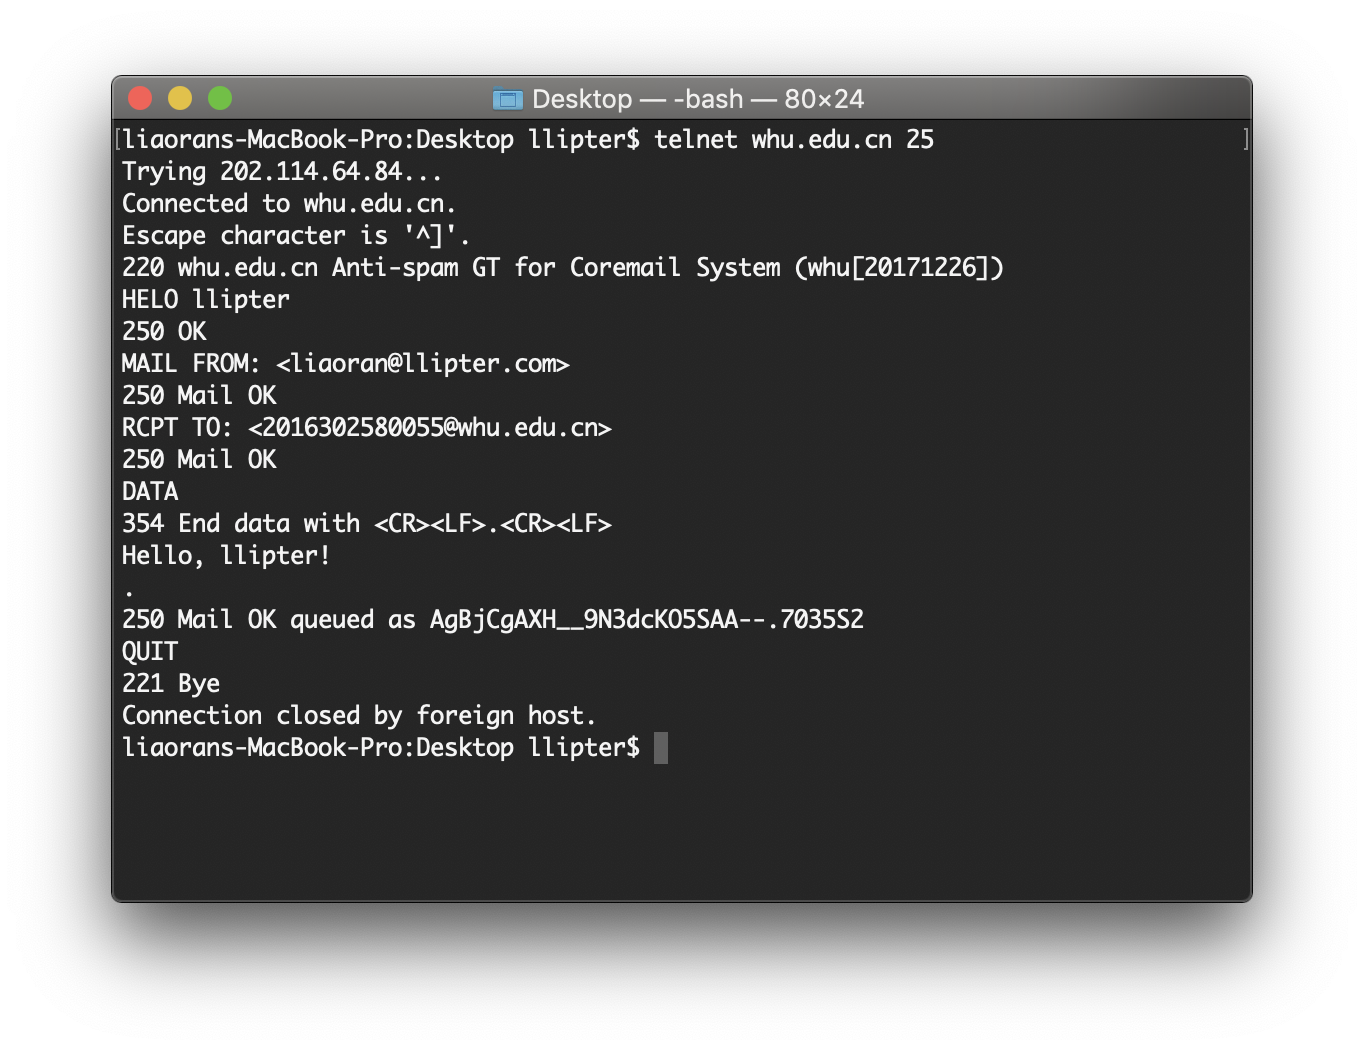
\includegraphics[width=1\textwidth]{telnet.png}
\caption{\label{fig:telnet}Telnet whu.edu.cn}
\end{figure}

\newpage
\section{Problem 1}

True or false?

\begin{qparts}

	\item \textbf{A user requests a Web page that consists of some text and three images. For this page, the client will send one request message and receive four response messages.}
	
	False. One response per request.
	
	\item \textbf{Two distinct Web pages (for example, www.mit.edu/research .html and www.mit.edu /students.html) can be sent over the same persistent connection.}

	True.x
	
	\item \textbf{With nonpersistent connections between browser and origin server, it is possible for a single TCP segment to carry two distinct HTTP request messages.}
	
	False. Nonpersistent connections will send only one object per connection.
	
	\item \textbf{The Date: header in the HTTP response message indicates when the object in the response was last modified.}
	
	False. The Date: header line indicates the time and date when the HTTP response was created and sent by the server. Note that this is not the time when the object was created or last modified; it is the time when the server retrieves the object from its file system, inserts the object into the response message, and sends the response message. 
	
	\item \textbf{HTTP response messages never have an empty message body.}

	False. This could happen when using conditional GET.

\end{qparts}


\newpage
\section{Problem 3}

\textbf{Assume you open a browser and enter http://yourbusiness.com/about.html in the address bar. What happens until the webpage is dis- played? Provide details about the protocol(s) used and a high-level description of the messages exchanged.}

~\\

DNS protocol is used to convert domain to IP address and HTTP protocol is used to communicate with the server. Both of them are in application layer. And in transportation layer, TCP and UDP is used.
	


\newpage
\section{Problem 4}

Consider the following string of ASCII characters that were captured by Wireshark when the browser sent an HTTP GET message (i.e., this is the actual content of an HTTP GET message). The characters <cr><lf> are carriage return and line-feed characters (that is, the italized character string <cr> in the text below represents the single carriage-return character that was contained at that point in the HTTP header). Answer the following questions, indicating where in the HTTP GET message below you find the answer.

~\\

GET /cs453/index.html HTTP/1.1<cr><lf>Host: gaia.cs.umass.edu<cr><lf>User-Agent: Mozilla/5.0 ( Windows;U; Windows NT 5.1; en-US; rv:1.7.2) Gec ko/20040804 Netscape/7.2 (ax) <cr> <lf>Accept:ex t/xml, application/xml, application/xhtml+xml, text /html; q=0.9, text/plain; q=0.8,image/png,*/*; q=0.5<cr><lf>Accept-Language: en-us,en;q=0.5<cr><lf>Accept- Encoding: zip,deflate<cr><lf>Accept-Charset: ISO -8859-1,utf-8;q=0.7,*;q=0.7<cr><lf>Keep-Alive: 300<cr> <lf>Connection:keep-alive<cr><lf><cr><lf>

\begin{qparts}
	\item \textbf{What is the URL of the document requested by the browser?}
	
	gaia.cs.umass.edu/cs453/index.html
	

	\item  \textbf{What version of HTTP is the browser running?}

	HTTP/1.1
	
	\item  \textbf{Does the browser request a non-persistent or a persistent connection?}
	
	Persistent connection.
	
	\item  \textbf{What is the IP address of the host on which the browser is running?}
	
	No such information in HTTP request.
	
	\item  \textbf{What type of browser initiates this message? Why is the browser type needed in an HTTP request message?}
	
	Mozilla/5.0. Given this message, the server can send different version of objects to different browser to improve performance.
	

\end{qparts}

\newpage
\section{Problem 4}

The text below shows the reply sent from the server in response to the HTTP GET message in the question above. Answer the following questions, indicat- ing where in the message below you find the answer.

~\\

HTTP/1.1 200 OK<cr><lf>Date: Tue, 07 Mar 2008 12:39:45GMT<cr><lf>Server: Apache/ 2.0.52 (Fedora) <cr><lf>Last-Modified: Sat, 10 Dec2005 18:27:46 GMT<cr><lf>ETag: ”526c3-f22-a88a4c80”<cr><lf>Accept- Ranges: bytes<cr><lf>Content-Length: 3874<cr><lf> Keep-Alive: timeout=max=100<cr><lf>Connection: Keep-Alive<cr><lf>Content-Type: text/ html; charset = ISO-8859-1 <cr><lf><cr><lf><!doctype html public ”- //w3c//dtd html 4.0transitional//en”><lf><html><lf> <head> <lf> <meta http-equiv=”Content-Type” content=”text /html; charset=iso-8859-1”><lf> <meta name=”GENERATOR” content=”Mozilla/4.79 [en] (Windows NT 5.0; U) Netscape]”><lf> <title>CMPSCI 453 / 591 / NTU-ST550ASpring 2005 homepage </title><lf> </head><lf> <much more document text following here (not shown)>

\begin{qparts}
	\item \textbf{Was the server able to successfully find the document or not? What time was the document reply provided?
}

	Yes. It's on Tue, 07 Mar 2008 12:39:45GMT.
	
	\item \textbf{When was the document last modified?}
	
	Sat, 10 Dec2005 18:27:46 GMT.
	
	\item \textbf{How many bytes are there in the document being returned?}
	
	3874
	
	\item \textbf{What are the first 5 bytes of the document being returned? Did the server agree to a persistent connection?}

	The first 5 byte is <!doc. And the server agree to open a persistent connection.

\end{qparts}

\newpage
\section{Problem 17}

Consider accessing your e-mail with POP3.

\begin{qparts}
	\item \textbf{Suppose you have configured your POP mail client to operate in the download-and-delete mode.}

	C: list 
	
	S: 1 498 
	
	S: 2 912 
	
	S: .
	
	C: retr 1
	
	S: blah blah ... 
	
	S: ..........blah 
	
	S: .
	
	C: dele 1 
	
	C: retr 2

	S: (blah blah ... 
	
	S: ...........blah) 
	
	S: .

	C: dele 2

	C: quit

	S: +OK POP3 server signing off

	
	\item \textbf{What is the total response time for the scenario illustrated in Figure 2.20?}
	
	C: list 
	
	S: 1 498 
	
	S: 2 912 
	
	S: .

	C: retr 1
	
	S: blah blah ... 
	
	S: ..........blah 
	
	S: .
	
	C: retr 2

	S: blah blah ...

	S: ...........blah

	S: .

	C: quit

	S: +OK POP3 server signing off

	
	\item \textbf{Suppose you have configured your POP mail client to operate in the download-and-keep mode. Using your transcript in part (b), suppose you retrieve messages 1 and 2, exit POP, and then five minutes later you again access POP to retrieve new e-mail. Suppose that in the five-minute interval no new mes- sages have been sent to you. Provide a transcript of this second POP session.}
	
	C: list 
	
	S: 1 498

	S: 2 912

	S: .

	C: retr 1

	S: blah ..... 
	
	S: ....blah 
	
	S: .

	C: retr 2

	S: blah blah ...

	S: ...........blah

	S: .

	C: quit

	S: +OK POP3 server signing off
	
	
\end{qparts}

\end{document}